


\section{Industrial challenges} 


Sedimentation of particles falling or rising under the action of gravity through a fluid is frequently used in a variety of industrial and natural processes, such as food processing, cosmetics, petroleum production, and environmental remediation. 
It is an efficient way to separate solid particles or droplets from the surrounding fluid. 
The clarification of waste water makes use of such a physics, the particles or droplets rise up due to buoyancy forces, afterward they are ejected from the mixture.
Even though numerous experimental and theoretical studies have been conducted on this topic, models are still very restricted and show a significant lack of accuracy. 
In the Perspective of reducing the cost and the environmental impacts of energy processes involving multiphase flows, IFP Energies Nouvelles and public funds, supply finance for the theoretical as well as for experimental research on multiphase flows.
Therefore, this PhD work focuses on the theoretical and numerical modeling of buoyant emulsion in the context of water waste treatment.  

Let us now take the example of two processes of interest for IFP Energies Nouvelles, highlighting their physical implications and key challenges.  


\subsection{Liquid-Liquid extraction}


The first process is liquid-liquid extraction, specifically the ``agitated'' liquid-liquid extraction process. 

The liquid-liquid separation process is a unit operation during which one or more solutes are transferred from one liquid phase (diluent or dispersed phase) to another liquid phase (solvent or continuous phase).
The solvent and diluent phases are either immiscible or partially immiscible.
The separation efficiency relies on the difference in solubility of the solute between the two phases.
Typically, the solvent is an aqueous phase, often water, while the diluent is an organic phase, such as a non-polar solvent like ether or kerosene.
As phase transfer is proportional to the concentration of interfaces between phases, small droplets are initially desirable to maximize the interfacial concentration.
At the end of the process, separating the diluent and solvent phases becomes the priority, thus, coalescence between droplets is promoted to enhance phase separation.

Among liquid-liquid extraction processes, we now delve into more specifics by considering the agitated counter-current extraction process, as illustrated in \ref{fig:liq-liq}. 
The schematic in \ref{fig:liq-liq} (middle) depicts the operation of the process.
The first step involves injecting the continuous solvent phase from the top of the column, while the dispersed phase (i.e., the feed solution containing the solute) is introduced through the bottom inlet (see \ref{fig:liq-liq}). 
In addition to the buoyancy forces that naturally cause droplets to rise, an artificial downstream flow of the continuous phase is generated because the outlet for this phase is located at the bottom of the vessel. 
This design increases the relative velocity between the phases, and prolongs the residence time of the droplets in the vessel, hence optimizing species transfer. 
As the droplets, which are less dense than the solvent, rise due to buoyancy, they pass through agitators (represented by gray circles in \ref{fig:liq-liq}(middle)). 
The agitators create turbulence and shear forces that break the droplets into smaller droplets, enhancing mass transfer efficiency between the two liquid phases. 
Finally, the processed continuous liquid exits at the bottom of the vessel, while the dispersed phase exits at the top after separation. 

As an illustration \ref{eq:liq-liq}(left) shows a typical laboratory reproduction of the liquid-liquid separation process. 
Here, the different layers of agitators used to create dispersion are visible. 
Additionally, \ref{eq:liq-liq} depicts a real-scale industrial process, which spans several meters in height, highlighting the significant scale difference between laboratory setups and industrial applications. 
\begin{figure}[h!]
    \centering
    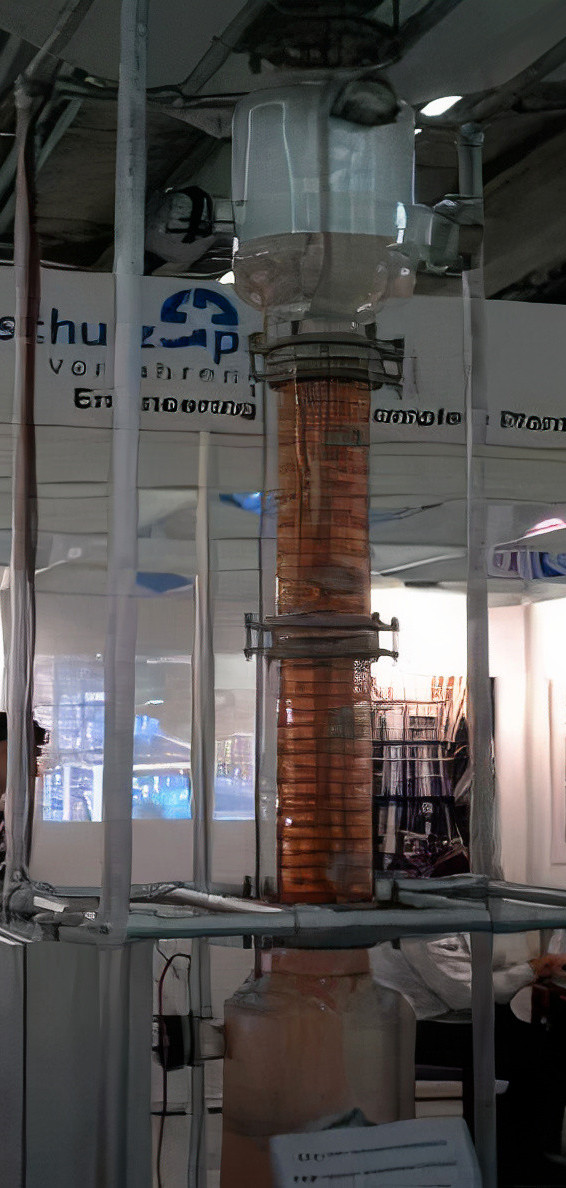
\includegraphics[height=0.3\textheight]{image/liq-liq_LE_auto_x5.jpg}
    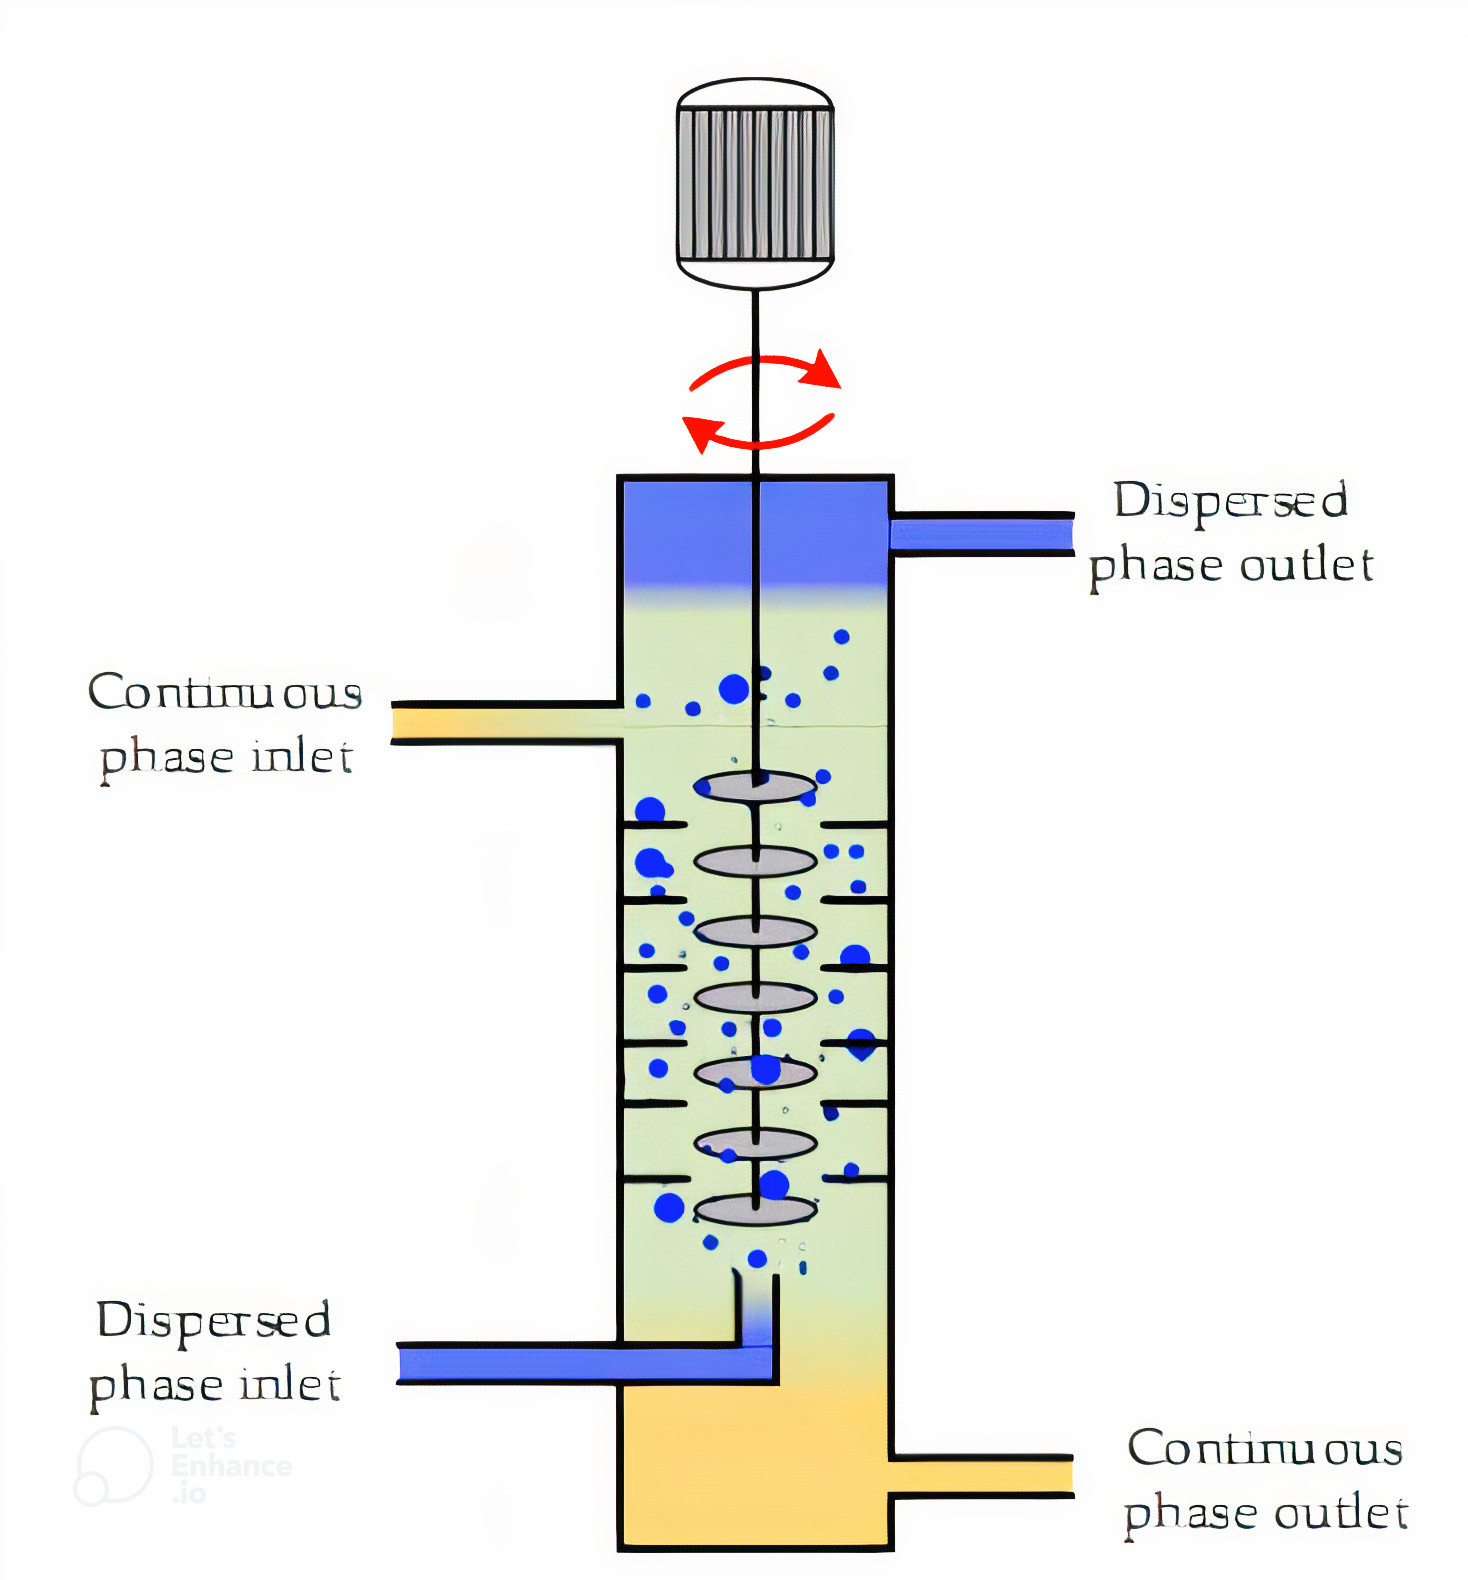
\includegraphics[height=0.3\textheight]{image/scheme_liq-liq_mieux.png}
    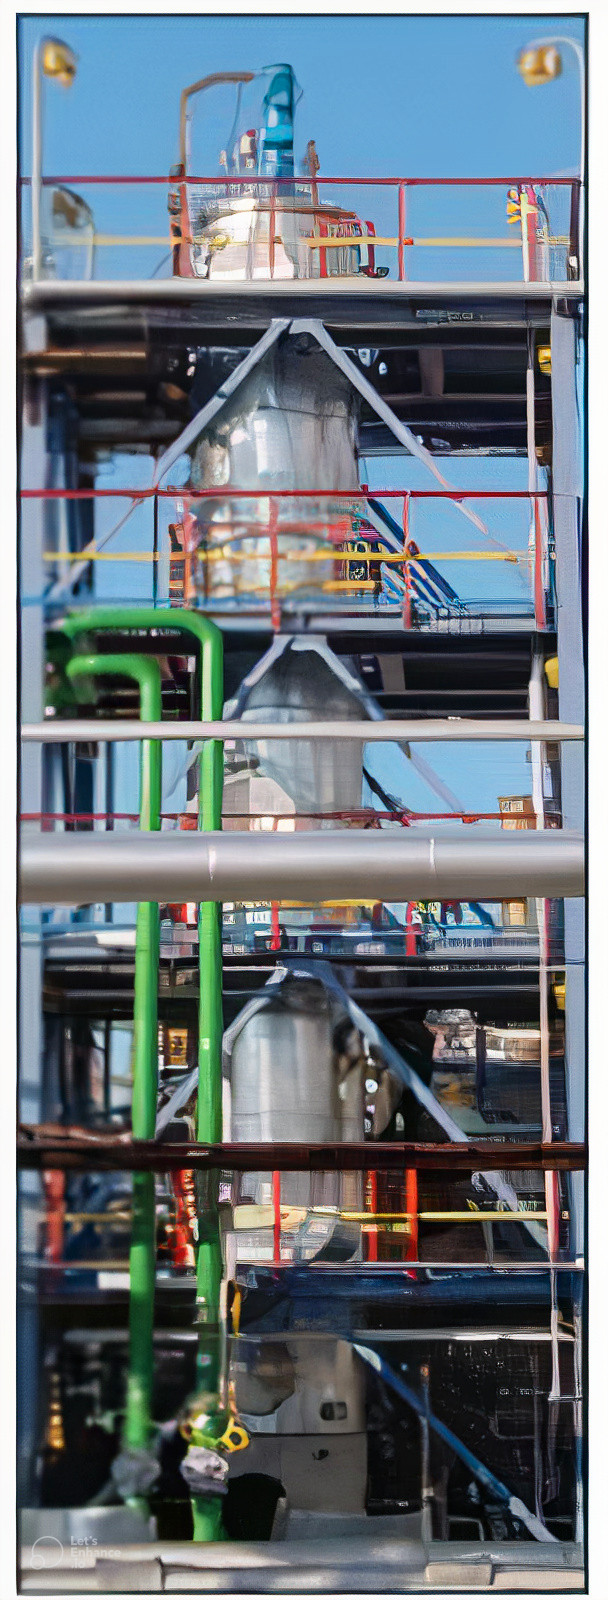
\includegraphics[height=0.3\textheight]{image/process_LE_auto_x4.jpg}

    % 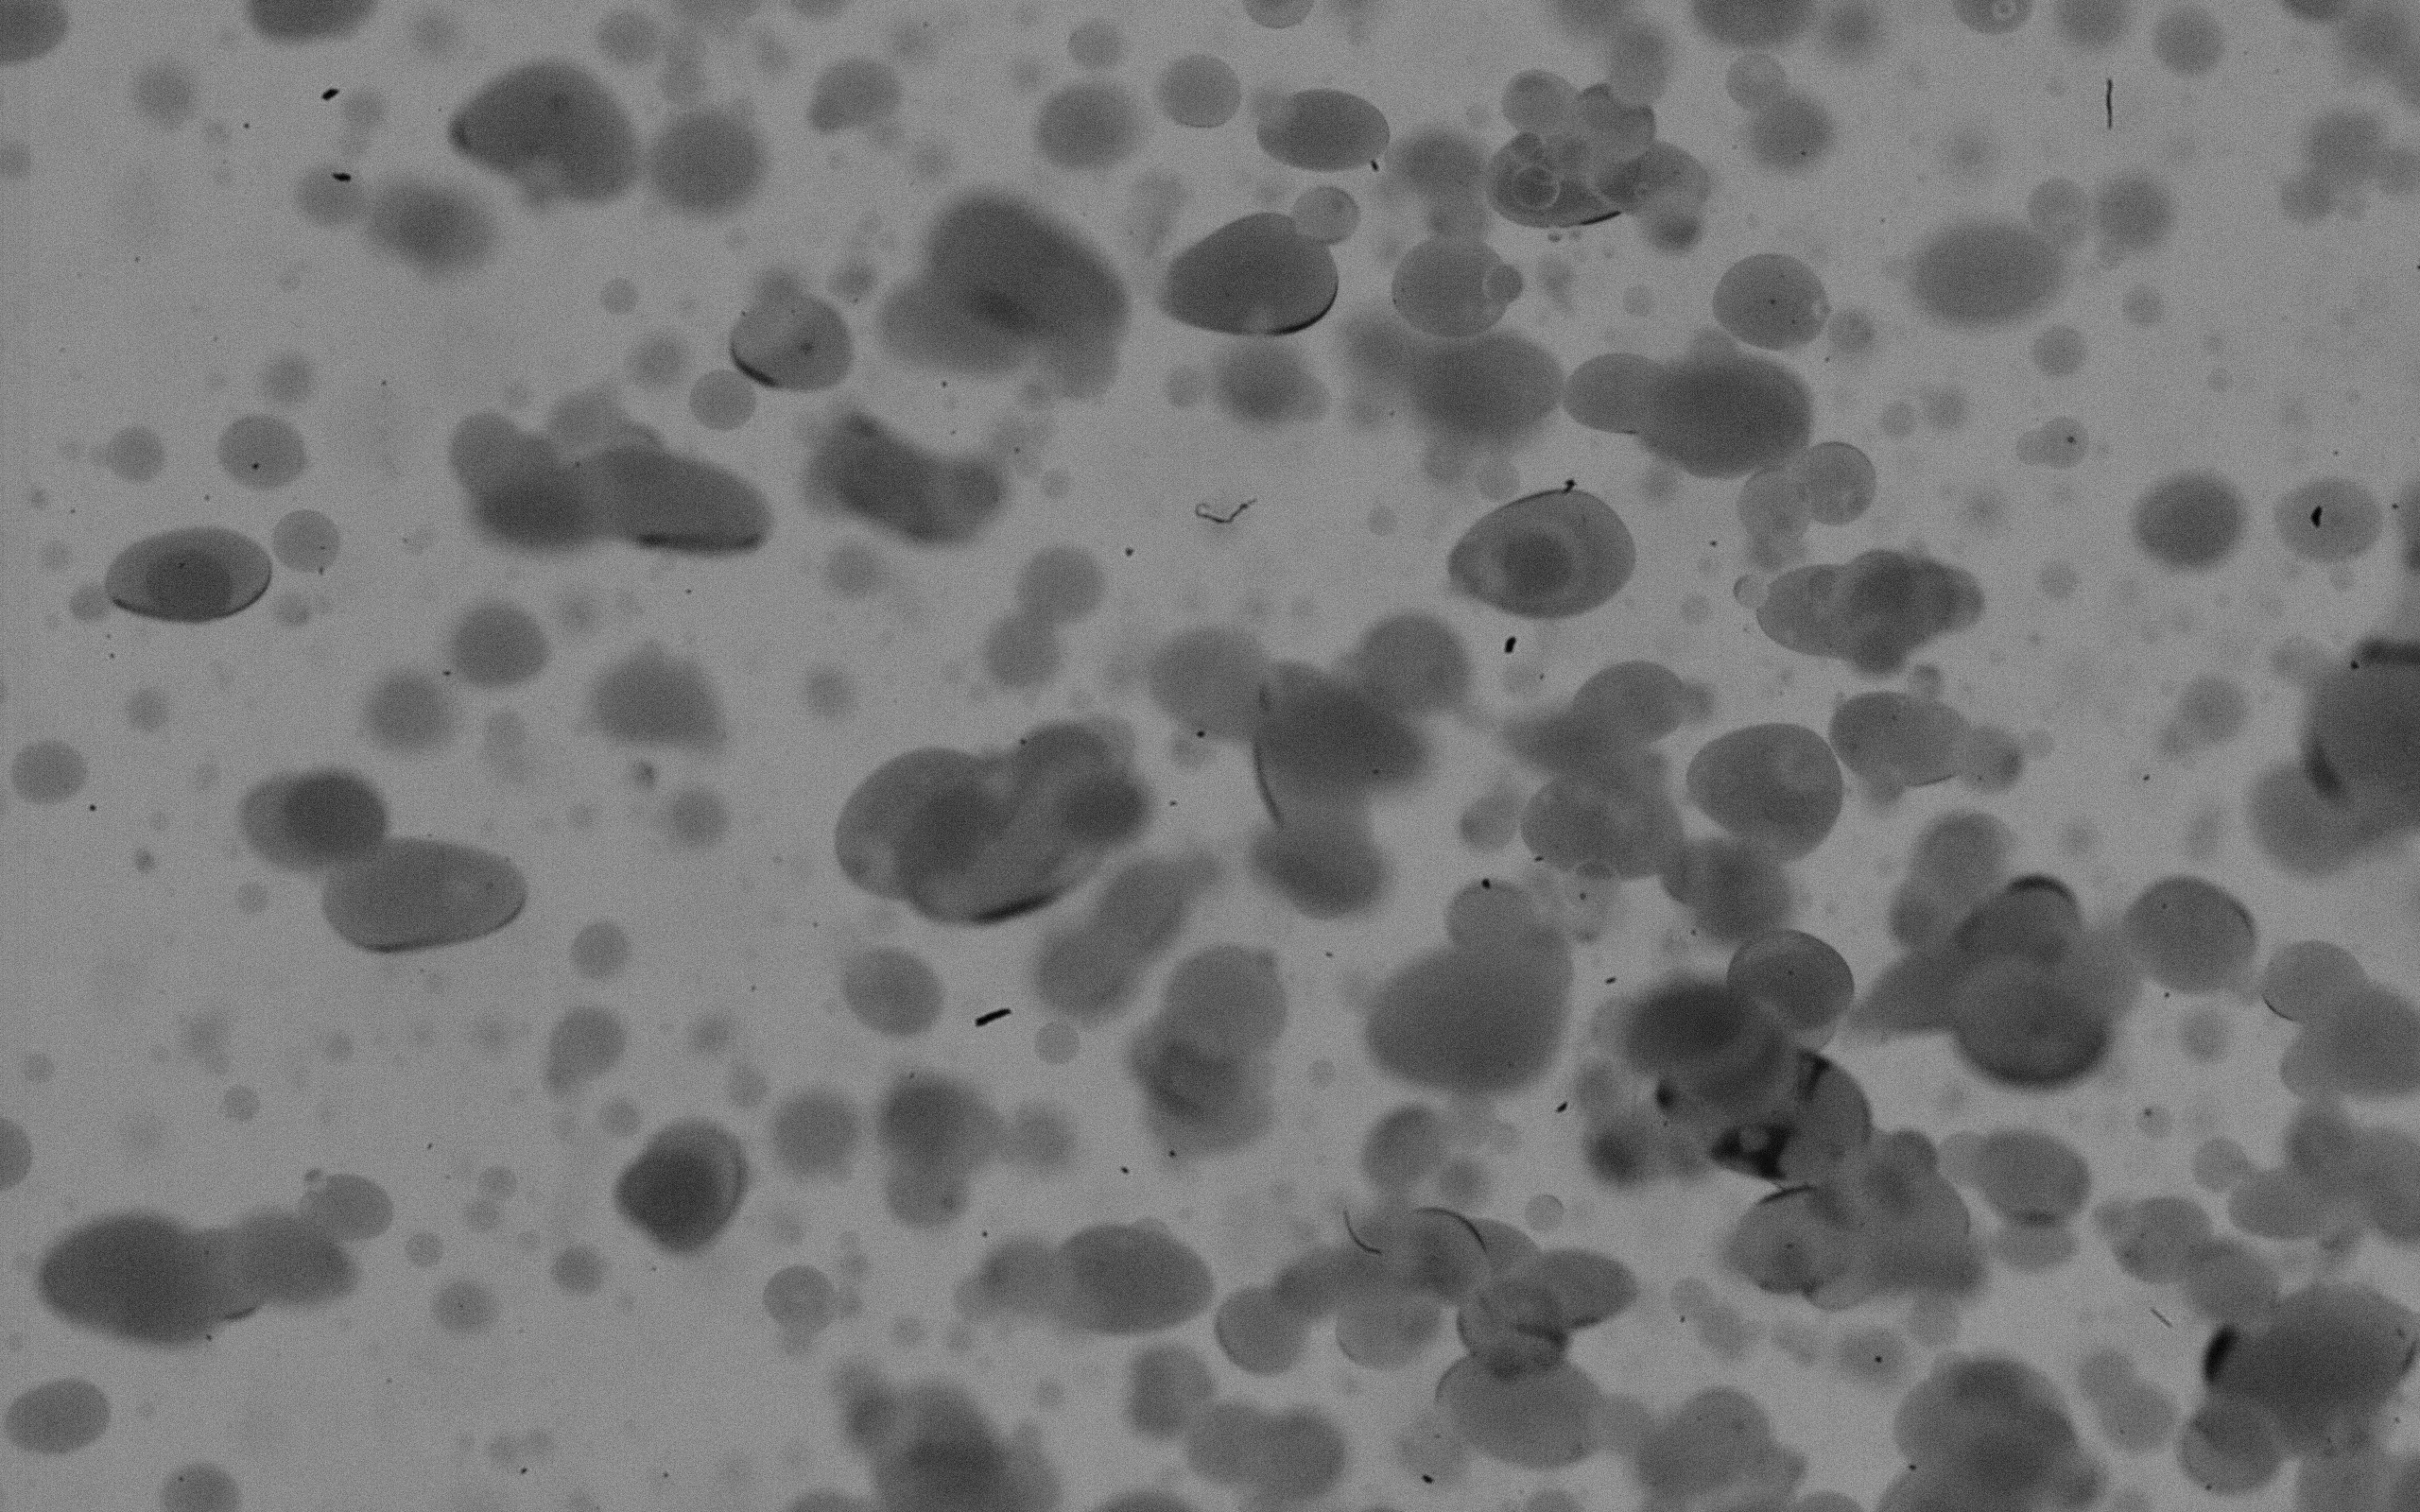
\includegraphics[height=0.15\textheight]{image/bubbles.png}
    \caption{
        (Left)   Pilot-scale illustration of the agitated liquid-liquid extraction process.
        (Middle) Schematic representation of the agitated liquid-liquid extraction process.
        (Right)  Industrial-scale liquid-liquid extraction process.
    }
    \label{fig:liq-liq}
\end{figure}



The aim of such a design is to transfer a species from one phase to another as efficiently as possible and subsequently to separate the diluent and solvent phases.
To achieve this, one must optimize the mass transfer rate between species based on hydrodynamic parameters, such as the operating conditions (e.g., input flow rates), the physical properties of the phases (e.g., density, viscosity, surface tension), and the geometry of the vessel and agitators.
Modeling such a process involves two major aspects.
(1) Thermodynamics modeling. This involves studying the migration of chemical species between the phases, including selecting suitable solvents and diluents to predict and optimize the separation efficiency of the mixture.
(2) Hydrodynamics modeling. This focuses on predicting the flow behavior of the continuous and dispersed phases within the vessel. Key considerations include determining the residence time of the droplets, their size distribution, and their relative velocity with respect to the solvent. These factors are crucial for accurately estimating the mass transfer rate within the vessel



As it will be important for the following discussion, let us specify the typical length scales involved in these processes:
(1) Macroscopic length scale: This corresponds to the size of the vessel, typically on the order of several meters $\sim 10 \text{m}$, as illustrated in \ref{fig:liq-liq} (right). 
(2) Hydrodynamic or Mesoscopic length scale: This is determined by the typical size of a droplet of diluent, which is approximately $\sim 1 mm$. 
(3) Nanoscopic length scale: If we examine the thermodynamic and chemical interactions occurring at the surface of the droplets, the relevant length scale is that of Van der Waals forces, which is approximately $\sim 1 nm$. 
As will be explained in more detail later, this extremely wide range of length scales makes the problem particularly challenging to analyze and model. 

To summarize, enhancing our understanding of the process requires characterizing and modeling the mass transfer in terms of both the local and global hydrodynamic properties of the flow within the vessel. 
This includes predicting the droplets' velocity distributions and size distribution. 
Such models can be developed through small-scale experiments, such as those conducted in the pilot-scale column (\ref{fig:liq-liq} (left)) or through numerical simulations, as will be presented in the following. 
Once the underlying physics is fully understood and predictable, the process can be optimized effectively.


\subsection{Flotation process}

Over 80\% of the world’s wastewater is released into the environment without treatment. 
This underscores the need to develop water treatment processes that are more efficient, compact, and energy-efficient. 
Among the various separation techniques employed in wastewater treatment, flotation represents a key method. 

The basic principle of flotation involves separating suspended inclusions in water, typically around $1\mu m$, by introducing air bubbles, approximately $\sim 1 mm$ in diameter, at the bottom of the vessel, see \ref{fig:flo} (left).   
As the bubbles ascend, they collide with the particles and eventually the particles get attached to the bubbles and rise with the bubble to the top of the vessel.
The waste particles, trapped within the foam formed by the bubbles at the surface, are then removed from the top of the vessel, leaving clear water behind.  
\begin{figure}[h!]
    \centering
    % 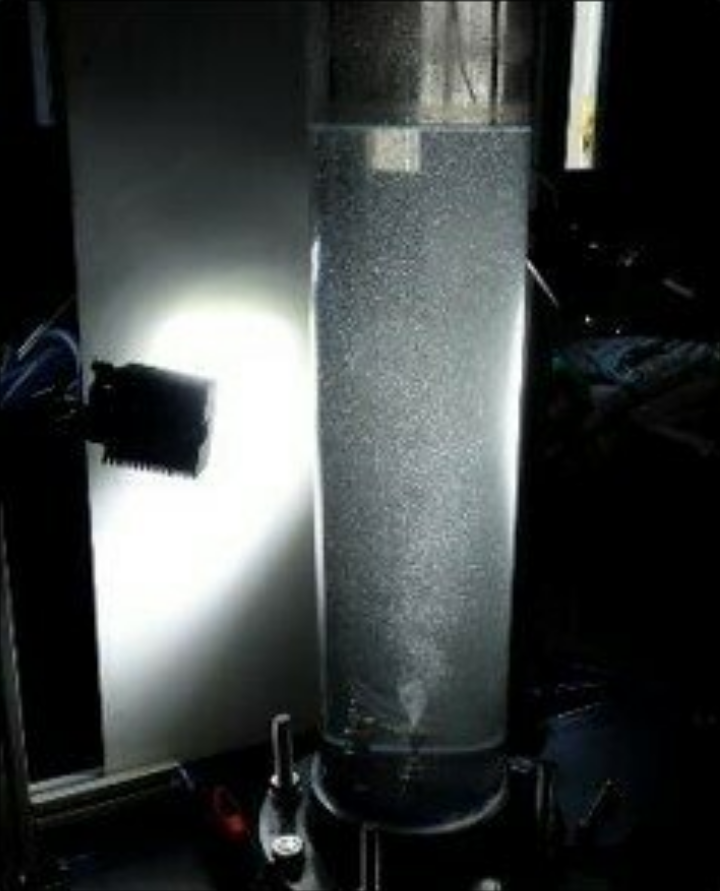
\includegraphics[height=0.3\textwidth]{image/flo.png}
    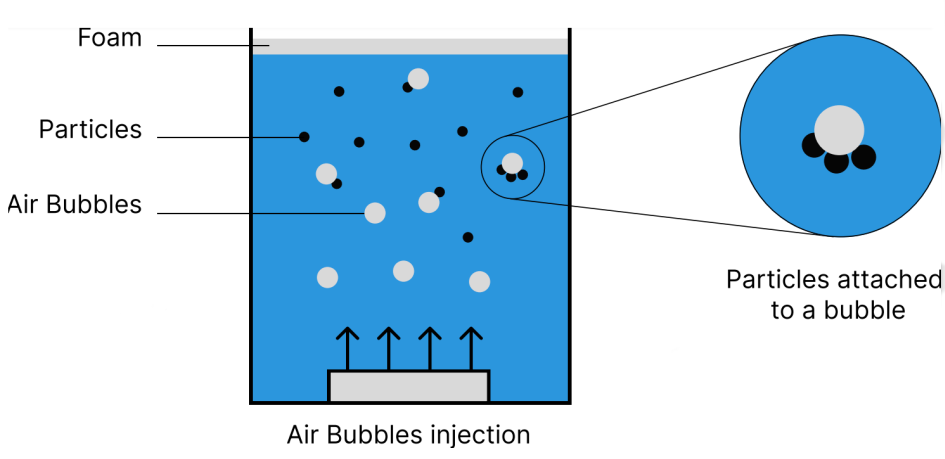
\includegraphics[height=0.3\textwidth]{image/flo_scheme.png}
    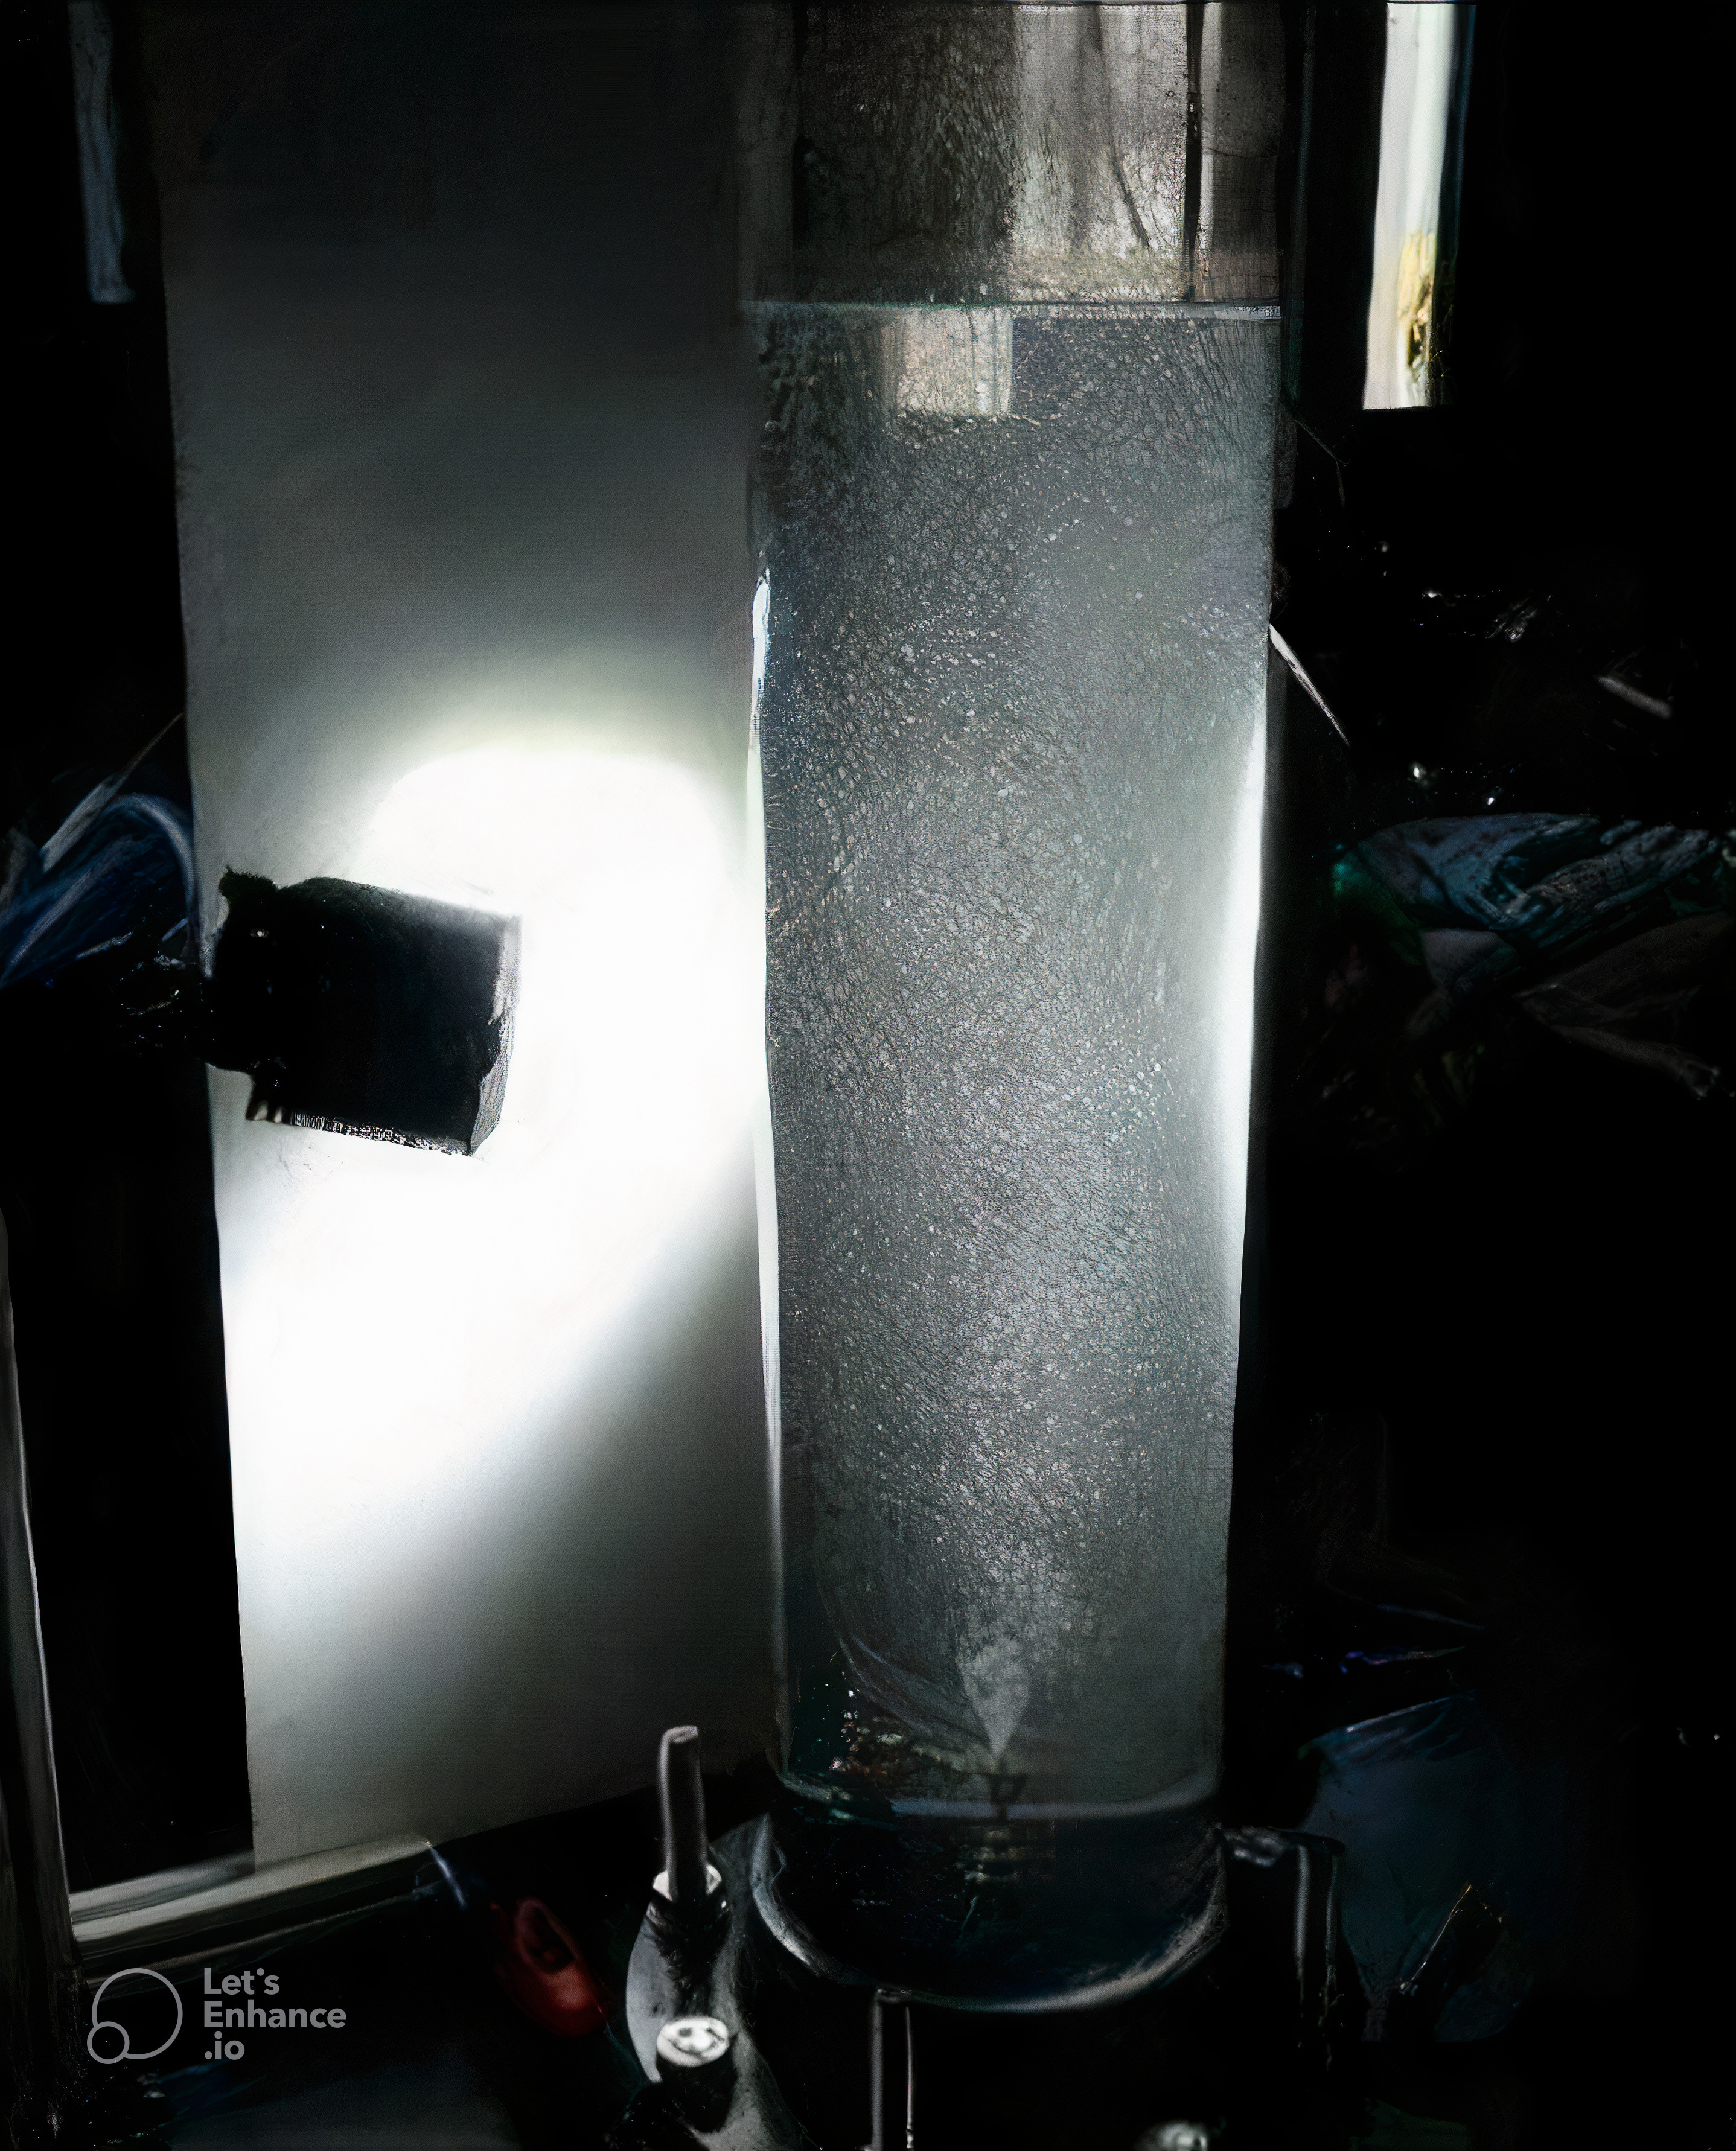
\includegraphics[height=0.3\textwidth]{image/flo_LE_auto_x4.jpg}
    \caption{
        (left) Scheme of the flotation column. 
        (right) Laboratory flotation column. 
        Reprinted from \citet{landal2025}
        }
        \label{fig:flo}
\end{figure}

For illustrative purposes, we present in \ref{fig:flo} (right) a typical flotation column experiment. 
This design aims to optimize the rate at which particles (i.e., water waste) attach to bubbles and are subsequently removed from the continuous water phase. 
To achieve this, it is crucial to predict the global hydrodynamics, which includes the interactions between the dispersed and continuous phases, as well as particle-bubble and bubble-bubble interactions.
The bubble-particle interactions play a fundamental role, as they determine whether or not a particle attaches to the bubble. 
These interactions depend on various factors, such as the size and surface properties of both the particle and the bubble, their relative velocities, and the surrounding flow conditions. 
Thus, in this process, the size distribution of the dispersed phases and their velocities play a pivotal role in determining the particle attachment rate to the bubbles.



To summarize, in order to model and optimize the flotation process, one must be able to accurately model the microscale interactions, such as the bubbles-particle interactions, across the entire vessel, which is typically on the order of several meters. 
Although the flotation process differs significantly from liquid-liquid separation, both processes share a common point: they involve modeling small bubbles, droplets, or solid particles immersed in a continuous phase that fills the vessel, with sizes on the order of $\sim 1000$ droplets-size. 
In this PhD work, we focus on modeling the interactions between droplets and the continuous phase, as well as between droplets themselves, while neglecting the interactions with smaller particles, for example. The multi-scale nature of both the flotation and liquid-liquid extraction processes presents a major challenge in their modeling.



\section{A multiscale problem} 


As mentioned above the liquid-liquid multiphase flows, and more particularly, dispersed multiphase flows, often involve multiscale physical phenomena. 
Indeed, at the vessel scale, the liquid-liquid mixture can be approximated as two homogeneous phases, with effective properties that account for the droplet behavior in an averaged manner \citet{jackson2000}.
Then, the macroscopic properties and the hydrodynamics of the mixture depend on the microscale properties and the local interactions driving the physics at these scales. 

In the context of droplets, these interactions can be categorized into two types. The first type involves the hydrodynamic interactions between the dispersed phase and the continuous phase. 
The scale of interest here is the droplet scale, which is also referred to as the mesoscale. 
The second type of interaction arises from van der Waals forces, which act at the molecular scale.
Indeed, when droplets come into contact, chemical interactions, influenced by the thin fluid film separating them, play a significant role. This film is so thin that microscale forces, such as van der Waals interactions, become non-negligible. Notably, the probability of two droplets coalescing upon contact is affected by these chemical interactions. As a result, these interactions impact the droplet size distribution, influencing behaviors at the droplet scale, which in turn affect mass transfer and attachment probabilities in processes such as liquid-liquid extraction and flotation.

Consequently, the macroscopic properties of the flow, which determine the global efficiency of the process, are a function of the local-scale properties of the flows.
This highlights the importance of understanding and modeling the multiscale nature of these flows to optimize and improve the processes.

To conclude, we can identify three scales in this problem:
(1) The macroscopic scale (macroscale): This is the scale of the vessel, where the medium is treated as a homogeneous mixture. 
At this scale, the entire flow can be approximated as a mixture of two-homogeneous flows with effective properties related to the dispersed and continuous phase which account for the behavior of the dispersed droplets and surrounding continuos phase.
(2) The mesoscopic scale (mesoscale): This scale concerns the individual droplets and the hydrodynamic forces that drive their motion and interactions. It involves studying the relative velocities between droplets and the continuous phase, as well as the interactions between droplets themselves.
(3) The molecular scale (microscale): At this scale, we focus on the chemical interactions that occur at the interfaces between droplets. This includes van der Waals forces, surfactant effects, and mass transfer at the droplet surfaces, all of which influence the coalescence behavior, droplet size distribution, and other microscopic phenomena. 
As mentioned, in these processes the chemical interactions also involve surfactant and mass transfer at the surface of the droplets.
Below, \ref{fig:scaling_up} schematizes the global multiscale strategy employed in this work to describe these types of multiphase flows.

\begin{figure}[h!]   
    \centering
    \begin{tikzpicture}[font=\footnotesize,very thick, scale = 0.9] 
        % \node (img0) at (-0.1\textwidth,-0.35\textwidth) {
\includegraphics[height=0.1\textwidth]{image/logo.png}};
        \node (img1) at (-0.35\textwidth,0.25\textwidth) {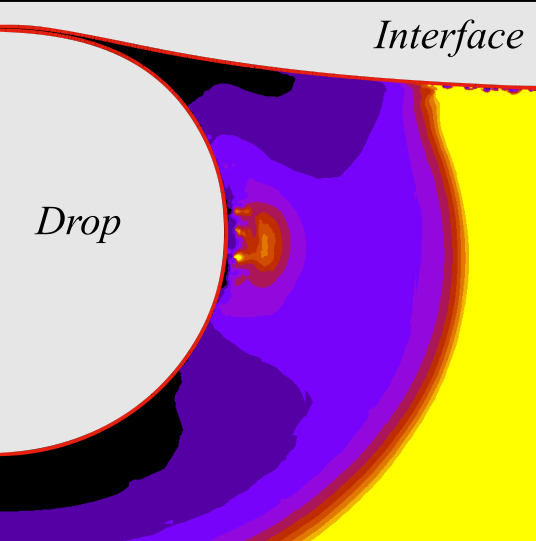
\includegraphics[height=0.25\textwidth]{image/film_drainage.png}};
        \node (img2) at (0\textwidth,0\textwidth) {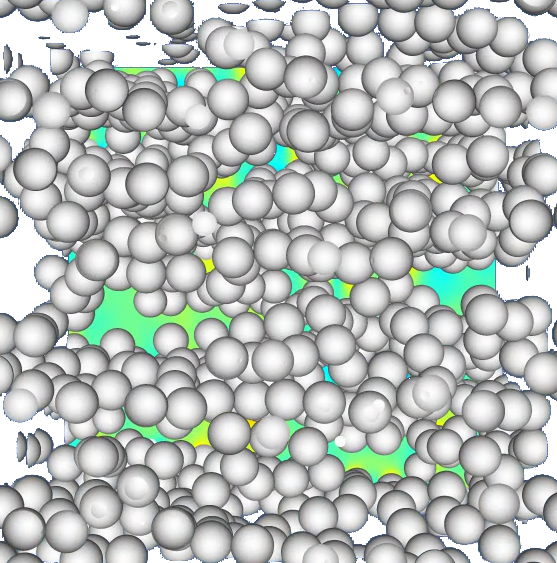
\includegraphics[height=0.25\textwidth]{image/700drop.png}};
        \node[very thick,fill=white,draw=gray] (ttx) at (0\textwidth,0.25\textwidth)
        {
        \begin{minipage}{4.4cm}
            Closure terms:
            \begin{itemize}[topsep=0pt, partopsep=0pt]
                \setlength{\itemsep}{0pt} 
                \setlength{\parskip}{0pt}
                \item \textcolor{red}{Interphase drag force}.
                \item \textcolor{red}{Velocity fluctuation}.
                \item Coalesence kernel.
                \item \ldots
            \end{itemize}
        \end{minipage}
        };
        \node[very thick,fill=white,draw=gray] (ttx2) at (0\textwidth,-0.35\textwidth)
        {
            \begin{minipage}{4.4cm}
                Constrained parameters:
                \begin{itemize}[topsep=0pt, partopsep=0pt]
                    \setlength{\itemsep}{0pt} 
                    \setlength{\parskip}{0pt}
                    \item Max volume fractions. 
                    \item Phase density ratio. 
                    \item Phase viscosity ratio. 
                    \item \ldots
                    % \item Frequency of collision. 
                    % \item Interaction forces.
                \end{itemize}
            \end{minipage}
        };
        \node (img3) at (0.35\textwidth,0.25\textwidth) {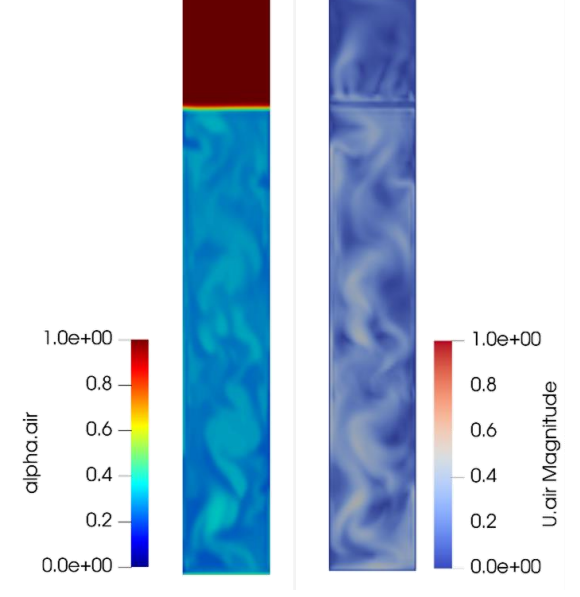
\includegraphics[height=0.25\textwidth]{image/Euler_Euler.png}};
        % \node (img4) at (0.425\textwidth,-0.25\textwidth) {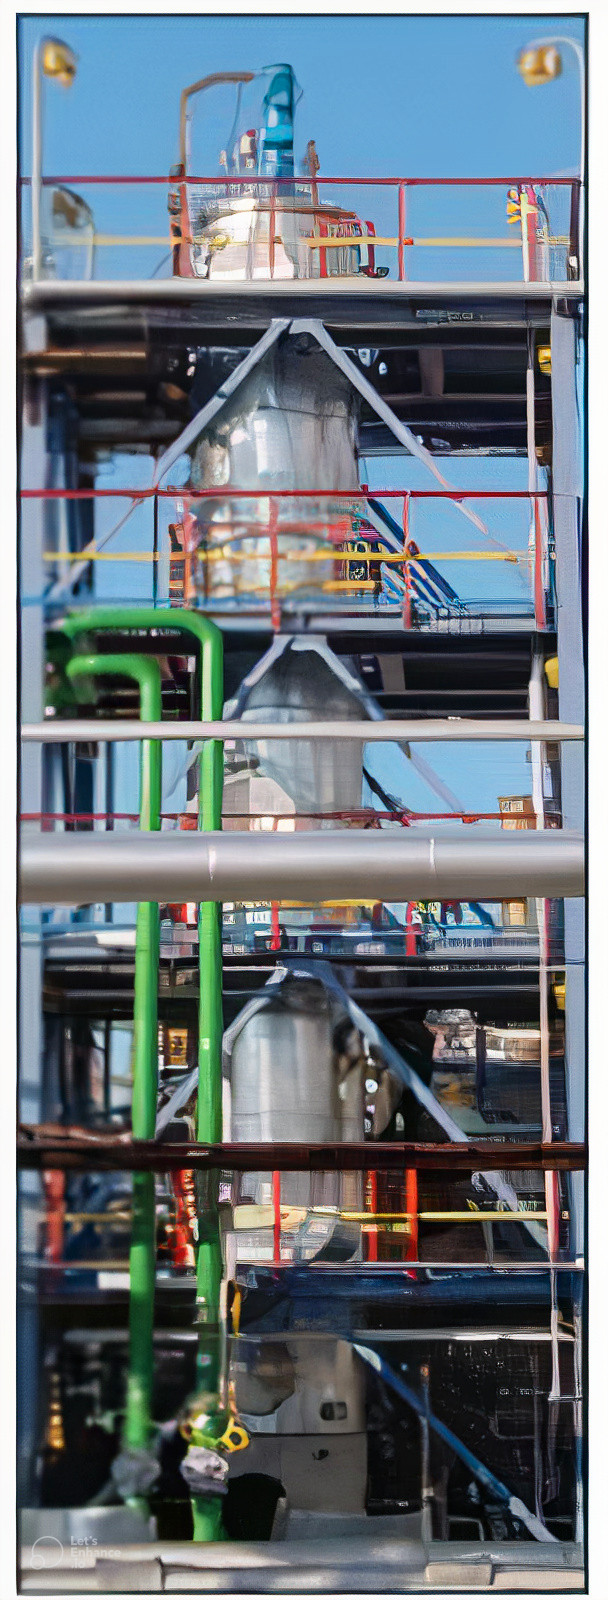
\includegraphics[height=0.25\textwidth]{image/process_LE_auto_x4.jpg}};
        \node (img4) at (0.35\textwidth,-0.25\textwidth) {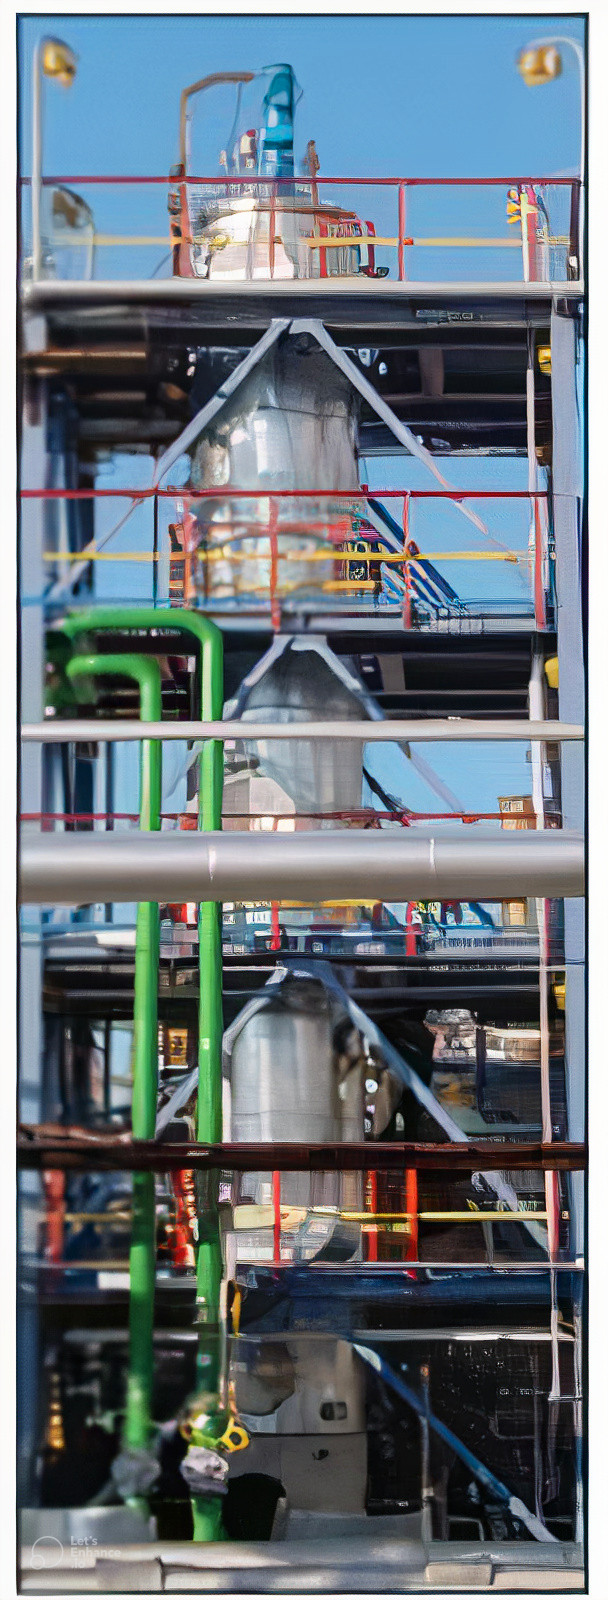
\includegraphics[height=0.25\textwidth]{image/process_LE_auto_x4.jpg}};
        %                   
        %                   
        %                   
        \node[align=center] (imgB) at (-0.35\textwidth,-0.48\textwidth) {\Large \underline{Film scale}};
        \node[align=center] (imgB) at (0,-0.48\textwidth) {\Large \underline{Particles scale}};
        \node[align=center] (imgB) at (0.35\textwidth,-0.48\textwidth) {\Large \underline{Process scale}};
        %
        \node[above,text width=0.3\textwidth] (imgC) at (img1.north) {Direct Numerical Simulation (DNS).};
        \node[below,text width=0.3\textwidth] (imgD) at (img2.south) {Particles Resolve Direct Numerical Simulation (PR-DNS).};
        \node[above,text width=0.3\textwidth] (imgC) at (img3.north) {Euler-Euler simulation of the processes. };
        \node[below,text width=0.3\textwidth] (imgC) at (img4.south) {Prototype / final product};
        %
        %
        \draw[->,very thick] (img1) -- (ttx.west);
        \draw[->,very thick] (img3) -- (img4)node[midway,fill=white,draw=gray]{
        \begin{minipage}{4.4cm}
            Optimized:
            \begin{itemize}[topsep=0pt, partopsep=0pt]
                \setlength{\itemsep}{0pt} 
                \setlength{\parskip}{0pt}
                \item Geometry of process. 
                \item Inter-phase transfer.
                % \begin{itemize}[topsep=0pt, partopsep=0pt]
                %     \setlength{\itemsep}{0pt} 
                %     \setlength{\parskip}{0pt}
                %     \item Thermique
                %     \item Chemical
                % \end{itemize}
                \item \ldots
            \end{itemize}
        \end{minipage}
        };
        \draw[->,very thick] (img2.north) -- (ttx);
        \draw[->,very thick] (img2) -| (img1)node[midway,fill=white,draw=gray]{
        \begin{minipage}{4.4cm}
            Constrained parameters:
            \begin{itemize}[topsep=0pt, partopsep=0pt]
                \setlength{\itemsep}{0pt} 
                \setlength{\parskip}{0pt}
                \item \textcolor{red}{Interaction kinematic}. 
                \item Frequency of collision. 
                \item Interaction forces.
            \end{itemize}
        \end{minipage}
        };
        \draw[->,very thick] (img4) -- (ttx2);
        \draw[->,very thick] (ttx2) -- (imgD);
        %
        \draw[->,very thick] (ttx.east) -- (img3);
        \draw[red,very thick] (img2.south west) rectangle(img2.north east);
        %
        \draw[very thin, dashed] (current bounding box.north)++(-0.175\textwidth,0) -- (-0.175\textwidth,0);
        \draw[very thin, dashed] (current bounding box.south)++(-0.175\textwidth,0) -- (-0.175\textwidth,0);
        \draw[very thin, dashed] (current bounding box.north)++(0.175\textwidth,0) -- (0.175\textwidth,0);
        \draw[very thin, dashed] (current bounding box.south)++(0.175\textwidth,0) -- (0.175\textwidth,0);
    \end{tikzpicture}
    \caption{Scaling up strategy of the processes' optimization.  The text in red and the red box represents the topics treated in this PhD. 
    Global description: 
    The process need to be modeled with averaged simulations; the averaged "Euler-Euler" simulations needs closures laws; these closure laws are provided by the film scale problem and particles scale problem; Both problem are drove by the parameter given by the upper-scale situation, which ultimately is the Prototype scale. }
    \label{fig:scaling_up}
\end{figure}

As one-to-one sized experiments of the processes are often too expensive to carry out, we aim to conduct numerical simulations based on ``averaged conservation laws'' that are valid at the macroscale. 
Another reason for this choice is the ease of measuring physical quantities that is afforded by numerical simulations, compared to real-life experiments, which often require invasive or inaccurate measurement tools.
Of course, throughout the optimization process, validation with experimental data will be necessary to ensure the reliability and accuracy of the simulation results. 
Note that these "averaged conservation laws" require models that account for the physics driving the meso- and microscale behavior of the flow. 
Thus, this PhD work primarily focuses on deriving the "averaged conservation laws" (discussed below) and on providing mesoscale models based on the study of the so-called mesoscale problem, namely, the multi-droplet interaction problem with the surrounding fluid.

\subsection{Mathematical modeling of dispersed two-phase flow}

Now, we would like to briefly present the methodology employed to derive these "averaged conservation laws," which will enable us to build numerical simulations of the above processes.
Before doing so we discuss a bit on kinetic-theory of Gases as the method to buid averaged equaitons for two-phase flows model is directly inspired from it. 

Note that multiphase flows can take several forms depending on the topology of the mixture. In this thesis, we focus on dispersed multiphase flows.
In this type of flow, the mixture consists of a continuous dominant phase, with inclusions dispersed within it. These inclusions can be of various natures, such as solid particles, liquid droplets, or gas bubbles.

\subsubsection{Links with kinetic-theory of gases}

We would like to begin our presentation with the smallest scale possible: the scale of the modeluces that constitutes a fluid or gas.
In a very simplistic approach, at this scale, molecules can be modeled as spheres colliding with each other. 
The behavior of a single molecule can be described using Newton's second law, which states that the sum of all forces acting on a particle is equal to its mass multiplied by its acceleration, $\textbf{F} = m \textbf{a}$. 
Essentially, this law allows us to predict the trajectory of one or several particles over time. 


To model a fluid or gas, essentially an ensemble of particles colliding with each other, Newton's second law becomes impractical due to the vast number of particles present in a unit volume of liquid or gas.
Thus, instead of modeling all individual particle trajectories, we derive equations for the average particle velocities and trajectories.
This is achieved through statistical methods, particularly the statistical kinetic theory of gases \cite{hansen2013theory,kardar2007statistical}.
For instance, the well-known Boltzmann equation describes the evolution of the one-point probability density function, representing the likelihood of finding a particle at a given location with a specific velocity.
Averaging this equation, multiplied by the velocity vector, leads to the Maxwell equations, which describe the balance of the averaged velocity of particles in a volume of fluid or gas.
These equations can be seen as the momentum balance for a fluid or gas.
It is important to note that they still represent the average velocity of all particles within the fluid.
Through this averaging procedure, fluids and gases, despite being composed of discrete particles, are viewed as continuous media at the microscopic scale.
Then, their specific behavior (Newtonian, non-Newtonian, shear-thinning, elastic, etc.) arises as a consequence of subscale interactions, which are captured through "constitutive laws" or "closure terms."
In other words, in the averaged equations describing the properties of the fluid, these closure terms represent the subscale physics that is needed to obtain a realistic model of the fluid.
By assuming the fluid is at thermodynamic equilibrium and exhibiting Newtonian behavior, for example, the equations governing fluid motion reduce to the Navier-Stokes equations. 

The main takeaway from this modeling approach is that, due to the vast number of particles in a parcel of fluid, we use probabilistic arguments to compute the averaged properties of the ensemble of particles, treating them as a continuum.
The upscaling strategy for modeling liquid-liquid separation and flotation processes follows a similar principle.
At a scale of approximately $1000$ droplet sizes, the Navier-Stokes equations—which themselves are averaged equations valid at the microscale—become computationally expensive to solve numerically.
To address this, we often rely on averaged equations that describe the mean motion of the dispersed and continuous phase.
This is referred to as the "two-fluid" model, initially developed by \citet{drew1983mathematical}.
In this framework, we require two sets of equations: one set to describe the dispersed phase (droplets or bubbles) and another to describe the motion of the continuous phase.
The parallel with kinetic theory can be extended further, as the centers of mass of the droplets or bubbles obey Newton's second law of motion, similar to the particles that constitute fluids and gases.


Thus, whether we aim to model numerous molecules or droplets, the procedure is essentially the same: we derive conservation laws for the averaged properties of an ensemble of particles (or droplets) rather than predicting the evolution of each individual particle (or droplet).
However, there is a notable difference between the modeling of molecules and two-fluid mixtures, beyond the obvious differences in size and shape between droplets and particles.
Molecules are typically assumed to evolve in void, interacting only with other molecules, while droplets interact continuously with the surrounding continuous phase and other droplets.
The predominance of droplet-continuous phase interactions over droplet-droplet interactions fundamentally changes the structure of the equations compared to the one governing the fluid at the microscale.
As a result, the methodology for deriving averaged two-phase flow equations differs significantly from that used in the kinetic theory of gases, nevertheless, the approach is conceptually similar.
Below, we describe in more detail the strategy employed to derive these averaged equations. 


\subsubsection{From the microscopic to the process scale}

Assuming that the Navier-Stokes equations govern the mesoscale motion in both the continuous and dispersed phases, we can derive the two-fluid averaged Navier-Stokes equations to model the macroscale motion of each phase. 
These averaged equations typically consist of the mass and momentum balance for the dispersed phase and the mass and momentum balance for the continuous phase. 
The unknowns in these equations include, for instance: The volume-averaged velocity of the continuous phase, $\textbf{u}_f$; The volume-averaged velocity of the particles $\textbf{u}_p$; The respective volume fractions of the continuous and dispersed phases, $\phi_f$ and $\phi_d$, respectively. 
To be representative, these equations require information about the sub-scales (i.e., the micro- and mesoscale dynamics).
As discussed above, the ``closure terms'' are mathematical expressions present in these averaged equations to account for the influence of subscale physics on the macroscale behavior. 
By ``mesostate'' we refer to the set of parameters describing the local properties of an emulsion at the droplet scale.
This includes:  droplet sizes, droplet shapes, droplet positions, droplet velocities, the velocity and pressure fields of the continuous phase around the droplets.
\footnote{
    The term ``mesostate'' is inspired by the concept of ``microstate'' commonly used in statistical mechanics, which refers to the instantaneous list of parameters describing the state of a system at the molecular level. Specifically, a microstate includes the molecules' positions and velocities at a given moment
    }. 
As an example, the closure terms can include the averaged drag force between the phases, the local velocity fluctuations, and the averaged Newtonian stress, all of which may be expressed in terms of the macroscopic unknowns ($\textbf{u}_p$, $\phi_d$, and $\textbf{u}_f$) to close the problem.
Consequently, solving these equations numerically requires a precise expression of the closure terms in terms of the macroscopic properties and, of course, an efficient solver to run the macroscale simulation and model the process.

The closure terms depend on what we call the probable ``mesostate'' of the flow. 
However, the existing ``mesostate'' can span an infinite phase space of parameters required to fully describe the local state of the continuous and dispersed phases.
It is clear that deriving an analytical expression of the closure terms valid for all possible ``mesostates'' is overly complex.
Therefore, studies are often limited to very specific situations to derive closure terms.
For example, it is often assumed that the dispersed phase consists of spherical particles and that the suspension is monodisperse, meaning all particles in the mixture have the same size.
In these simplified scenarios, some authors have successfully closed the averaged two-fluid Navier-Stokes equations theoretically.
For example, \citet{jackson1997locally} derived an averaged set of equations for a monodisperse suspension of solid spherical particles, where the closure terms were obtained under the assumption that the relative motion between the dispersed and continuous phases follows the Stokes equations. 
Similarly, \citet{zhang1997momentum} developed a set of averaged equations for a mono-disperse emulsion of spherical droplets, with the closure terms derived within the context of Stokes flow as well.


The preceding authors considered monodisperse suspensions; however, another crucial challenge for averaged equations is the modeling of the local size distribution of droplets within a given volume containing the emulsion.
The size distribution can be influenced by the migration of particles which posses different rising velocities due to their size variations, and by coalescence and breakup phenomena, which are governed by mechanical and chemical interactions.
As previously mentioned, the particle size distribution is of significant importance because it directly impacts mass transfer, and the probability of attachment which are crucial properties that we need to predict for the above processes.
The modeling of polydisperse flows involves the use of what are called Population Balance Equations (PBE), a related but distinct system of equations than the two-fluid averaged Navier-stokes equations.
A comprehensive review of polydisperse flow modeling is provided by  \citet{marchisio2013computational}. 


To summarize, we have demonstrated that modeling the above processes involves using averaged conservation laws that require "closure terms." These terms account for the mesostate and microstate behaviors of the emulsion. 
This upscaling methodology avoids the computational expense of directly solving the detailed flow and chemical interactions throughout the entire vessel.
To construct models, one must first study the interactions between multiple droplets and the continuous phase. 
In a second step, it is necessary to examine droplet-droplet interactions more closely to better predict coalescence and, consequently, the size distribution within a given emulsion.
These investigations require a combination of theoretical, numerical, and experimental data, which ultimately lead to the development of models and a comprehensive understanding of the multiscale problem. 

The problem of droplet-droplet interactions leading to coalescence can be addressed either experimentally or by employing Direct Numerical Simulation (DNS) to model the flow within the thin film between two droplets (see \ref{fig:scaling_up} (left)).
These DNS simulations must account for both the chemical interactions and the flow field within the thin film separating the two interfaces.
To model the interaction between multiple droplets and the continuous phase, we can use Particle-Resolved Direct Numerical Simulation (PR-DNS) \citep{tryggvason2006direct}, (see \ref{fig:scaling_up} (right)).
This approach is similar to DNS, however, it does not fully resolve the flow within the film between two interacting particles.
Indeed, accurately solving the flow around hundreds of droplets while also resolving the flow within the film during droplet collisions would be computationally too expansive.
In \ref{fig:scaling_up}, we display a schematic representation of the global strategy explained here.




\subsubsection{Hierarchy of the mathematical formulation to model dispersed two-phase flow}

Now we would like to provide a general picture of the different methodology employed to model dispersed flows, whether it is for two-fluid flows or for granular material or (as it is the case in kinetic theory) molecules. 
On \ref{fig:diagram} we represent these different modeling strategy with books of reference for each cathegory. 
Firstly, we can identify two main area on \ref{fig:diagram}, namely, the ``Lagrangian-'' and ``Eulerian-'' based models. 
The former correspond to the models that use Lagrangian laws to describe the dispersed phase evolution, and that are then averaged to obtain a macroscopic equations. 
In opposition the ``Eulerian-based model'' use an ``Eulerian'' approach to describe either the continuous or dispersed phase, and then we employ an average procedure to derive the macroscopic equaitons. 
Our classification identified four main categories, ``Kinematic-Theory'' models, ``Population-Balance-Model'' (PBE or PBM), ``Euler-Euler Two-fluid models'' (or just ``two fluid models''), and finally the ``hybrid models''. 
% \begin{figure}[h!]
%     % \begin{tikzpicture}[thick, scale=0.5]
%     \centering
%     \begin{tikzpicture}[thick, scale=1, every node/.style={scale=0.45}]
%         \node (img) at (0,0){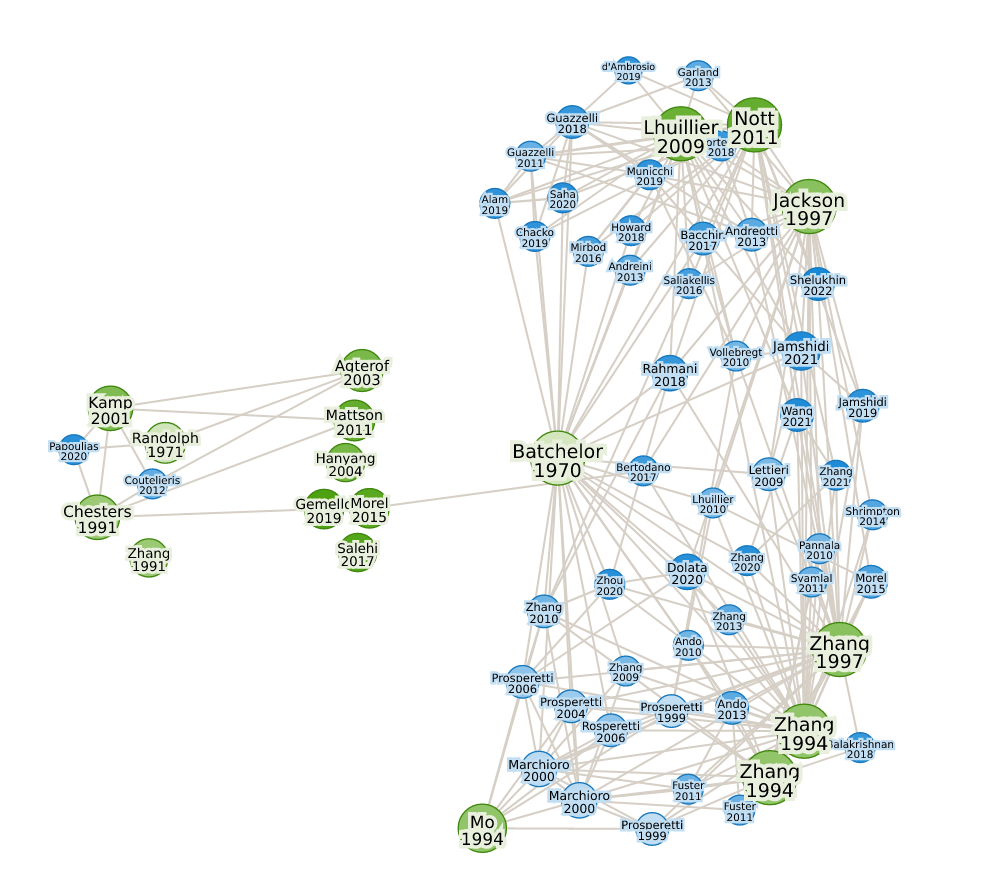
\includegraphics[width=2\textwidth]{Bib/graph70_paperGraph_network.png}};
%         \draw[dashed,very thick](-2,-0.5)ellipse(1 and 2.5);
%         \draw[dashed,very thick](-5,-0.5)ellipse(1.5 and 2.5);
%         \draw[dashed,very thick](4,4)ellipse(2 and 1.5);
%         \draw[dashed,very thick](4.5,-4)ellipse(1.5 and 2);
%         \draw[dashed,very thick](4,5)node[above,very thick]{\Large$\textbf{(III)}$};
%         \draw[dashed,very thick](6,-5)node[right,very thick]{\Large$\textbf{(II)}$};
%         \draw[dashed,very thick](-6.5,2)node[above,very thick]{\Large$\textbf{(I)}$};
%         \draw[dashed,very thick](-1.3,1.75)node[above,very thick]{\Large$\textbf{(IV)}$};
%         % \draw[<->](com2.north)--(com3.south)node[midway]{Equivalent};
%     \end{tikzpicture}
%     \caption{Non-exhaustive cartography of the different publications on population balance models and averaged equations. The articles are represented by the name of the first author. The lines between each article mean that both articles cited each other.}
%     \label{fig:carte}
% \end{figure}
\begin{figure}
    \centering
    \begin{tikzpicture}[node distance=10pt,font=\footnotesize]
    \tikzset{
        venn box/.style={
          draw=black, very thick, 
          rounded corners=10,
          inner xsep=10pt, inner ysep=15pt, outer ysep=5pt
        },
        venn numbers/.style={
      %    draw,
          inner ysep=0pt,
          align=center
        },
        venn title/.style={
          fill=black, text=white
        }
      }            
    \node[venn box,fill=gray!5] (N) {%
        \citet{rao2008introduction}
    };
    \node[venn numbers, above=of N] (Z-N) {
        \citet{marchisio2013computational}
    };
    \node[venn box, fit=(Z-N) (N) ] (Z) {};
    \node[venn numbers, above=of Z, align=center] (Q-Z) {};
    \node[venn box,fill=gray!5] (Q) at (5.5,0) {
        \citet{morel2015mathematical}
    };
    \node[venn numbers, right=of Q, inner sep=0pt, align=center] (Q-two) {
        \citet{drew1983mathematical}
    };
    \node [venn box, fit= (Q) (Q-two)] (R) at (6.5,0) {};
    \node [venn box, fit=(R),gray,dashed,inner ysep=50pt] (El) {};
    \draw[gray] node[fill=white,anchor=north west] at ([shift={(10pt, 3pt)}]El.north west) {Eulerian-based models};
    \node [venn box, fit=(Q) (Z) ,gray!50,dashed] (D) {};
    \draw[gray!50] node[fill=white,anchor=north west] at ([shift={(10pt, 3pt)}]D.north west) {Lagrangian-based models};
    \tikzset{every node/.style=venn title}
    \draw node[anchor=north east] at ([shift={(-10pt, 3pt)}]R.north east) {Two-fluids model};
    \foreach \i/\j/\k in {N/Kinetic-Theory/0, Z/PBE/10pt, Q/Hybrid model/10pt} {
        \draw node[anchor=north west] at ([shift={(10pt, 3pt)}]\i.north west) {\j};
              %node[rounded corners] at ([yshift=-\k]\i.east) {${\i}$};
              }

      \end{tikzpicture}
    \caption{Mathematicla modeling of dispersed two phase flows carthorgraphy. Lagrangian-based model: correspond to the averaged model derived by averaging Lagrangian governing laws on each particles contituing the dispersed phase. 
    Eulerian-based model: correspond to the averaged model derived by averaging the Eulerian governing laws valid within each phase of the flow. }
    \label{fig:diagram}
\end{figure}


The area denoted by ``Kinetic-Theory'' represent the studies dedicated to the modeling of Gases and liquid \citep{hansen2013theory} through kinetic-theory. 
Note that the basic model consider solid spherical mono-disperse assembly of particles  \citet{kardar2007statistical}.
Kinetic-Theory can also be used to describe elongated particles \citet{curtiss1956kinetic,hansen2013theory}, which is useful to model material constituted with orientable structure of molecules.
The description of matter is the origin of kinetic theory however it can also be used to describe more macroscopic phenomena such as granular materials \citet{rao2008introduction}.  

The classical use of Kinetic-Theory consider mono-disperse assembly of particles. 
Extending this theory to poly-disperse assembly of particles and one obtain the so-called Population-Balance-Equaitons. 
The only aspect that changes is that PBE includes equations to be solved for the probability distribution of the particle size or its moments \citep{fox2023generalized}. 
\citet{randolph2012theory} introduced the first population balance models, at the origin it was designed  for Crystallizes. 
A good review of the PBE model can be found in \citet{marchisio2013computational}. 
The former two modeling approaches focused mainly on the modeling of the dispersed phase.
The continuous phase (when there is one) is treated by averaging the Eulerian conservation laws of the fluid. 
However, the mathematical relation between the dispersed phase and continuous phase is made somewhat empirically since both phases equations are derived independently. 
That is the reason why the Kinetic-Theory and PBE models are not included in the ``Eulerian-based'' models. 

Let us focus on a liquid-liquid system such as emulsion. 
In this case the majority of averaged two-fluid models derived to model such flow are based on the framework proposed by \citet{drew1983mathematical}, where both the dispersed and continuous phases are derived by averaging the local Eulerian conservation law governing the fluid in each phases, see \ref{fig:diagram}.
Despite its versatility-allowing applications beyond dispersed flows, such as stratified or slug flow, the physical interpretation of the closure terms remains difficult \citep{drew1983mathematical}.
Additionally, properties that are relevant for our processes optimizasion such as droplets-size distribution cannot be determined with such a modelisation since ``Two-fluids models'' do not assume any topology for the dispersed phase.
Nevertheless, one advantage of this model compared to the former one regarding the modeling of dispersed flows, is that the exchanges terms within the equations of the dispersed phase and continuous phase are ``well-connected''. 

Consequently, to model emulsion, we need a model  which is able to describe the topology of the flow, such as size the size distribution of droplets, their deformation and so on, and that is properly linked with the continuous phase, so that the global set of equations remain consistent. 
Such a model is termed ``Hybrid model'' since it is a Lagrangian- / Eulerian- based model.
The difference with the previous model is that the Eulerian exachang terms in of the continous phase equaitons are termed into Lagrangian-based exchange terms, which makes the whole system consistent. 

Many previous studies that used the "hybrid" formalism have focused on solid particles \citep{buyevich1979flow,jackson1997locally}. 
Notable exceptions include \citet{zhang1994ensemble}, who investigated spherical bubbles with time-varying radii, and \citet{zhang1997momentum}, who examined spherical droplets. 
Despite these advancements, the question remains: how can different inclusion shapes, internal fluid motion, and surface transport equations be incorporated into such Lagrangian models? 
To the best of our knowledge, important surface properties , such as variable or constant surface tension, the arbitrary shape of fluid particles, and the distribution of surfactants, have not yet been fully incorporated into current averaged hybrid models.  
% While the Lagrangian formulation of the interfacial area equation is well established \citep{lhuillier2000bilan}, its application to define general Lagrangian quantities for a dispersed phase is still not fully explored. 
A good review of the ``hybrid model'' for bubbly flow can be found in \citet{morel2015mathematical}. 
Anyhow, it seems that there is a need for a comprehensive hybrid model that encompasses all relevant physical aspects, including surface properties and arbitrarily shaped particles.

Overall a model relating kinetic-theory-like equations while taking in account the fluid nature of the particles seems absence from the state of the art. 
In this manuscript we propose a general framework able to describe a dispersed phase of arbitrary nature with surface properties while being consistent with the kinetic-theory-like model.

\subsection{Lake of theoretical and empirical models}

Eitehr it is for PBE, Kinetic-Theory, Two-fluid or Hybrid  models, one needs accurate closure terms to represent the closures terms. 
In this work we classified the closure terms into three groups. 


The first group represents the closure terms that are common to any particles type. 
For example, the momentum exchange term, the Reynolds stress or pseudo-turbulent stress, appear in every averaged model, regardless of the dispersed phase nature and topology. 
Hence, numerous studies have already develop accurate model for these closures. 
Nevertheless, while an enormous amount of work have been devoted for solid particles and bubbles, less work have been provided to build model for emulsion. 
Particularly, the viscosity ratio between the dispersed phase and continuous phase needs to be included as input of these model that either consider one of these extreme.

The second group corresponds to the closure that appear solely because the dispersed phase is made of fluid inclusion. 
This includes, the internal particle kinetic energy, the internal dissipation etc \ldots
% For example the internal viscous dissipation within the droplets is a closure term.
These terms appear in the equations only because we will consider an ``hybrid'' formulation of the averaged equations, and because the dispersed phase is made of fluid particles. 
As mentioned above, the ``hybrid'' formulation treating fluid particles are not common. 
Hence, these closure terms are either not known from the community or rarely studied. 
Thus, a clear lake of understanding to models these new terms is present.  

The third and final group is the PBE-related closure terms. 
These include the coalescence and break-up kernels that act as source term in the size-distribution equaiton. 
There is an extensive body of literature on coalescence. 
A review of this literature can be found in the works of \citet{chesters1991modelling}. 
However, due to the multi-physics and multi-scale nature of the problem, there is currently no predictive model that has achieved consensus in the literature. 
Thus, even if enormous effort have been devoted to the development of these kernels, major advancement still remain to be done. 



\subsection{Ambition and objectives of this PhD.}




As the complete problem constitutes an enormous task this PhD focuses on two main aspects: 
(1) The mathematical modeling of dispersed two-phase flow, this includes the development of a more complete ``hybrid model'' adapted to the modeling of emulsions; and (2) the numerical modeling of the PR-DNS simulation to feed this ``hybrid model''. Note that the closure terms are restricted to mono-disperse stead-state buoyant emulsion. 

Additionally, in this work we study only the modeling of the momentum and mechanical energy related equation-and closure terms. 
Meaning that we won't dive into the chemical aspect of the problem that is needed to model the liquid-liquid extraction processes. 
We also restrict our selves to the Particle-scale modeling, hence we won't dive into the film-drainage problem and its modeling.   
Nevertheless, we still provide indispensable information regarding the ``Constrained'' or ``input'' parameters that are useful for the film drainage problem. 

In \ref{fig:scaling_up} we present a diagram that summarize to whole modeling strategy of this PhD work. 
The text and the box colored in red represent the aspect of the problem treated in this manuscript. 


\section{Outline of the manuscript}


In order to provide a consistent methodology to derive averaged equations and useful closure terms to feed the former equations we partitioned this manuscript into three main parts. 

\paragraph*{Part I: } 
The first part focus on the mathematical modeling of dispersed two phase flows, that is the derivation of the averaged equaitons as well as the derivation of the closure problem. 

The first chapter, (\ref{chap:daniel1}), provides a derivation of the averaged equations governing the motion of dispersed two-phase flows with interfacial transport. 
We begin by revisiting the two-fluid formulation, as well as the distributional form of the interfacial transport equation which holds on the entire domain. 
Following this, a general Lagrangian model is introduced, which accounts for the effects of both internal and interfacial properties of the dispersed inclusions (bubbles, droplets, or particles) within a continuous phase.
We then proceed by deriving the lesser-known conservation equations for the moments of the volume and surface distribution of an arbitrary Lagrangian property.
The paper concludes by presenting a ”hybrid” set of equations, consisting of phase-averaged equations for the continuous fluid phase, complemented by an arbitrary number of moment conservation equations for the dispersed phase.
The goal of this chapter was to provide the most general approaches to derive averaged equation so that the reader obtain a wide understanding of the mathematical structure of these equations. 

\ref{chap:daniel15} we expose the minimal set of equations necessary to describe emulsions made of Newtonian droplets based on the ``hybrid'' formulation developed in the \ref{chap:daniel1}. 
In short, we expose the ensemble-averaged momentum and energy equations in the ``hybrid'' formalism for arbitrary Newtonian droplet including surface tension properties. 
Notably, this derivation allowed us to discuss the energy exchange present in a dispersed two-phase flow. 
Additionally, we provided an explicit and general formulation for the effective stress in an emulsion. 

Finally, in \ref{chap:deformable} we decide to focus on the modeling of rising ellipsoidal droplets. 
We propose a set of equations that use the hybrid model to describe ellipsoidal rising droplets' droplet. 


\ref{chap:daniel2} we demonstrate how to re-formulated the closure term of the averaged model into conditionally averaged equations. 
Then, we demonstrate how to derive the corresponding conditionally averaged equations. 
This methodology is inspired from \citet{hinch1977averaged} and generalized.
After deriving the closure problem itself we derive the closure terms for spherical droplets in stokes flow.  




\paragraph*{Part II: } 
\ref{part:one} was purely theoretical, hence in \ref{part:two} we introduce Particle Resolve Direct-Numerical Simulation (PR-DNS) of buoyant emulsion in a tri-periodic domain. 
These simulations are conducted using the open source library \texttt{Basilisk C}.
These will serve as a basis to compare with the subsequent theoretical investigation and extend the validity of the models.  

In \ref{chap:closure-disperse} we solve the conditionally averaged equations in the dilute and Stokes limit to provide theoretical models for the closure terms of the ``hybrid-model''. 
Following the study of \ref{chap:deformable} we also consider the effect of finite inertia on rising ellipsoidal droplets.
The effective stress of the suspension is also investigated in this case.  


In \ref{chap:mono-disperse} we develop a model for the inter-phase drag force present in the averaged momentum equations. 
Based on the theory and simulation results we were able to construct a complete model for the inter-phase drag force taking in account an arbitrary ratio of viscosity between phases, volume fraction of droplets and Reynolds number based on the relative velocity between phases. 

In \ref{chap:pseudoturbulence} we focus on what is called the Reynolds stress tensor, that is the variance of the local continuous phase velocity. 
This velocity fluctuation tensor can be produced by the relative motions of the droplets with the continuous phase (that is the wake of the droplets), and other sources of turbulence. 
In this chapter we only focus on the former contribution and build a Model taking in account the dispersed phase volume fraction, relative velocity between phases and viscosity ratio between phases. 



\paragraph*{Part III:} 
The last part  focus on the study of the relative interaction between droplets among the emulsion. 


In \ref{chap:microstructure} we characterize the particles relative position of the droplets, that is termed the study of the microstructure of the emulsion. 
This is done using the nearest-neighbors distribution of the droplets in the emulsion. 

In \ref{chpa:microstructure_kin} we then study the relative velocity between particles, that is the study of the kinematic of the microstructure. 
The motivation for these  chapters is to provide useful information for the understanding of how in average pair of droplets interact together. 




Finally, we end this manuscript with a chapter on the perspectives and conclusions. 